\section{Process}
Our process has been a loosely coordinated heuristic process. Using the fact that the group had only two members and that the members were familiar with working together allowed us to dispense with a formal group structure and to handle all coordination in weekly meetings and through conversation. The group used discord to facilitate communication and github for version control of the source code.\\

An initial roadmap was made before beginning the development, where the overall stages in the process was marked out and give an expected duration(see figure \ref{fig:iterate}). The roadmap was made as a first estimate of the steps required to answer the problem statement. 

\begin{figure}[h]
\centering
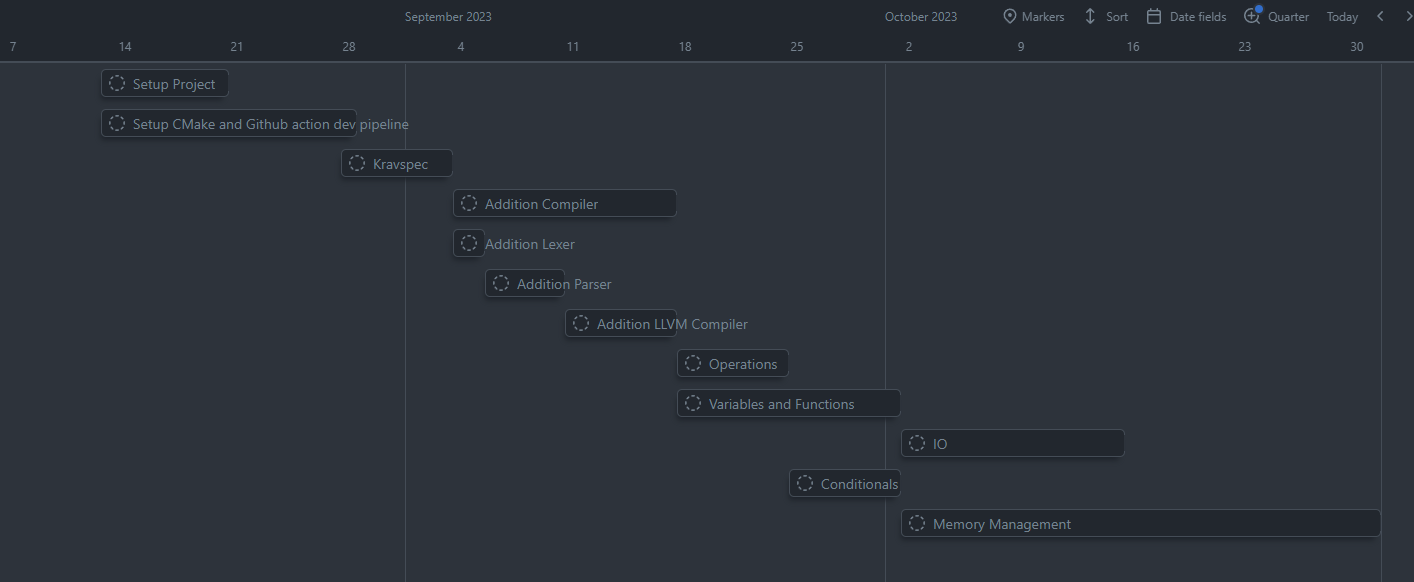
\includegraphics[width=\textwidth]{02-Body/Images/Roadmap.png}
\caption{Initial roadmap for the project}
\label{fig:iterate}
\end{figure}

The iterative process consisted of weekly meetings, where the current state of
development was reviewed, and future work discussed and planned. To determine which tasks should be focused on in the next iteration, we considered what would be the smallest step towards answering the problem statement, while leaving us with a 'finished' product at the end. This could be tasks such as:
\begin{itemize}
  \item Implement the Type Checker for the current state of \lang{}.
  \item Implement Function calls
\end{itemize} 

With this approach we always had a working product, and if something did not work out
as expected, only one or at most two weeks of work was lost. The roadmap illustrates
that the majority of the development was done as two parallel tasks. This was done to
maximise the work done, minimize duplicate work, and avoid merge conflicts in git.

\newpage
